\chapter{Drugs}
\label{chap:Drugs}

\section{Amphetamine-related stimulant drugs}


Amphetamine-related stimulant drugs -- including {\bf methylphenidate}
(Ritalin), {\bf amphetamine} (Adderall, Dexedrine), \& {\bf methamphetamine}
(Desoxyn) -- are commonly prescribed for children from as young as age 3.

Adderall is an amphetamine pharmaceutical that contains 25\% levoamphetamine
salts and 75\% dextroamphetamine salt.


\subsection{methylphenidate}
\label{sec:methylphenidate}

USE: ADHD and narcolepsy.

Methylphenidate's mechanism of action involves the {\it inhibition} of
catecholamine reuptake (Sect.\ref{sec:Catecholamines}), primarily as a {\it
dopamine reuptake inhibitor}.
Methylphenidate acts by blocking the dopamine transporter and norepinephrine
transporter, leading to increased concentrations of dopamine and norepinephrine
within the synaptic cleft.

NOTE: Methylphenidate is also a weak 5HT1A receptor agonist
(Sect.\ref{sec:serotonin-receptors}), i.e. reduce cAMP production
(Sect.\ref{sec:cAMP}).


As methyphenidate is effective in treatment ADHD, current models of ADHD
suggest that it is associated with functional impairments in some of the brain's
neurotransmitter systems, particularly those involving dopamine and
norepinephrine.

The use of the drug on normal healthy adults showed modest yet unambiguous
improvements in cognition, including working memory, episodic memory, and
inhibitory control. The cognition-enhancing effects of these drugs are known to
occur through the \textcolor{blue}{indirect activation of both dopamine receptor
D1 and adrenoceptor $\alpha$2 in the prefrontal cortex}.


\section{-- Methamphetamine (METH)}
\label{sec:methamphetamine}

Methamphetamine (METH) enters the brain via blood stream, it stimulates the DA
neurons whose activation links to bringing pleasure
(Sect.\ref{sec:METH-target-DA-neurons}).

Methamphetamine is {\bf double methylated phenylethylamine},
Fig.\ref{fig:amphetamine}(B).
The double (-NH2) process is the primary difference between amphetamine
(Sect.\ref{sec:amphetamine}) and methamphetamine in a laboratory or scientific
instance, i.e. methamphetamine is neurotoxic to humans, damaging both dopamine
and serotonin neurons (Sect.\ref{sec:serotonergic-neuron}) in the CNS, but not
inducing DA cell death.

Methamphetamine was discovered in 1893 and exists as two enantiomers:
{\bf dextromethamphetamine} and {\bf levomethamphetamine}.
NOTE: {\it racemic free base} is an equal mixture of levomethamphetamine and
dextromethamphetamine in their pure amine forms.
    
\begin{enumerate}
  \item 2008: methamphetamine (METH) used associated with 66,000 emergency room
  visits (SAMHSA, 2010)
  
  \item repeated use and high doses of METH associated with 
  \begin{itemize}
    \item cognitive  (Gonzalez et al., 2004; Scot et al., 2007)
    \item structural  (Chan et al., 2007)
    \item neurochemical  (Wilson et al., 1996)
  \end{itemize}
  abnormalities.
  
\end{enumerate}

\subsection{target DA neurons}
\label{sec:METH-target-DA-neurons}

METH induces dopaminergic effects through blockage and reversal of dopamine
transporter (DAT - Sect.\ref{sec:dopamine-transporter}), i.e. leading to
increase level of [DA] in extracellular space, and subsequent free redical
production (?????)
% TODO: find out mechanism of dopamine to free radical production Yamamoto and
% Zhu 1998

METH's effect is pronounced in striatum (Change et al., 2007); while amphetamine
affect DAT in the NAc (Sect.\ref{sec:nucleus_accumbens}) (Wise and Bozarth,
1995).

Chronic METH users exhibit deficits in 
\begin{itemize}
  \item  glucose metabolism (Wang et al., 2004)
  
  \item DAT density (Sect.\ref{sec:DAT}), dopamine content, and activity of
  rate-limiting enzyme tyrosine hydrolase (Wilson et al., 1996).Sect.\ref{sec:Catecholamines}
\end{itemize}

\subsection{Dopamine transporter (DAT)}
\label{sec:dopamine-transporter}
\label{sec:DAT}




\subsection{dose}

Methamphetamine HCL is dissolved in saline at a concentration of 15 mg/mL.

\subsection{Side effects}

Methamphetamine is a drug that can induce different side effects:
\begin{verbatim}
    Impaired speech
    Rapid pulse
    Dry mouth
    Shallow breathing
    Constipation
    Dizziness
    Insomnia
\end{verbatim}

\section{-- Amphetamine}
% \chapter{Amphetamine}
\label{chap:amphetamine}
\label{sec:amphetamine}

Although both amphetamines and methamphetamine (METH -
Sect.\ref{sec:methamphetamine}) do have many of the same characteristics and
qualities, they are both stimulants and they are both dangerous, they are not
exactly the same.

\begin{figure}[hbt]
  \centerline{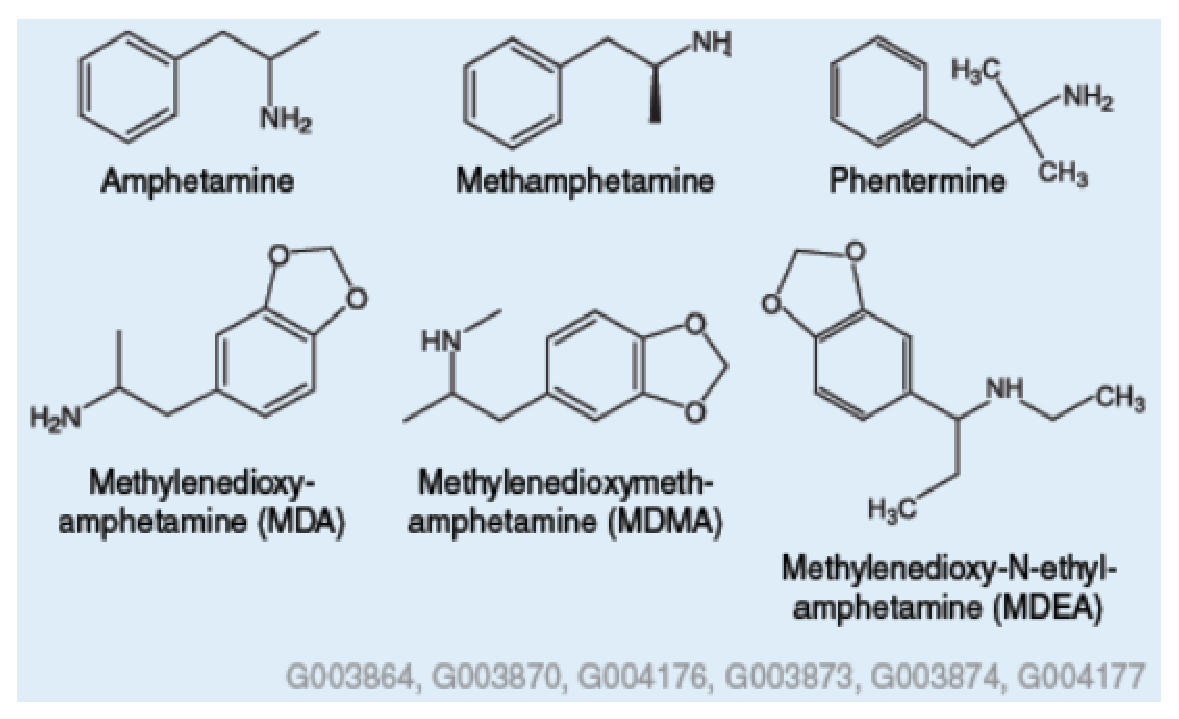
\includegraphics[height=5cm,
    angle=0]{./images/amphetamine.eps}}
  \caption{Amphetamine; Methamphetamine; Phentermine; MDA; MDMA; and MDEA}
\label{fig:amphetamine}
\end{figure}

When properly used, amphetamine is a powerful drug that can have many uses -
methamphetamine on the other hand does not have many uses besides recreational
drug use. The effects of amphetamine are very strong and this can lead to an
increased metabolism, rapid heart rate and similar effects.

Amphetamine is scientifically known as {\bf methylated phenylethylamine}.
Methamphetamine is {\bf double methylated phenylethylamine}. The double process
is the primary difference between amphetamine and methamphetamine in a
laboratory or scientific instance.

Amphetamine was discovered in 1887 and exists as two enantiomers:
{\bf levoamphetamine} and {\bf dextroamphetamine}.

What it does?
\begin{enumerate}
  \item sensitize NMDAR on D1-MSN: - Sect.\ref{sec:amphetamine-D1-MSN}
  
  \item 
\end{enumerate}

\section{Cannabis plant}
\label{sec:cannabis}
\label{sec:tetrahydrocannabinol}


Unlike morphine (Sect.\ref{sec:morphine}), marijuana/cannabis creates opposite
effect to the brain, i.e. causing euphoria which is about the opposite of
depression.

Tetrahydrocannabinol (THC, the active ingredient in {\bf
marijuana})) was found (in mid-1960s) as the primary psychoactive component 
produced by Cannabis plant that bind to receptors known as cannabinoid receptors
(Sect.\ref{sec:cannabinoid-receptors}), one of that is CB1-R. 

The psychoactive effects of THC are primarily mediated by its activation of
CB1-R (Sect.\ref{sec:CB1R}).

\begin{enumerate}
  \item  common marijuana contains 2 to 5\% THC, while 
  
  \item ganja can contain up to   15\% THC and 
  
  \item hashish oil between 15 and 60\%   THC
\end{enumerate}


There is a recent call for using cannabis as a better choice rather than opioids
in pain relief as it does not increase the  likelihood of abusing alcohol or
other drugs.

Some studies suggest the combination of cannabis with opiates may have a
synergistic effect.
\url{https://www.leafly.com/news/science-tech/the-medical-minute-cannabis-and-opioids/}

\subsection{THC}
\label{sec:THC}
 
Delta-9-tetrahydrocannabinol ($\Delta$9-THC, THC) and
delta-8-tetrahydrocannabinol ($\Delta$8-THC), mimic the actions of anandamide
and 2-arachidonoylglycerol, neurotransmitters produced naturally in the body
(Sect.\ref{sec:neurotransmitter}).

\begin{enumerate}
  \item partial agonist to CB1-R (Sect.\ref{sec:cannabinoid-receptors}), mainly
  in CNS; and CB2-R mainly in cells of immune systems.
  
  CB1-R: $K_i$ = 10 nM
  
  CB2-R: $K_i$ = 24 nM.
  
  
  \item 
\end{enumerate}

\subsection{Marijuana}
\label{sec:marijuana}


Marijuana and other derivatives of the plant {\it Cannabis
sativa} have been used for thousands of years for their
therapeutic and mood-altering properties.
Strangely cannabis was used widely for medicine thousands of years before opium
but they were both discovered about the same time, 4000 B.C. 

The main active ingredient of marijuana is THC (Sect.\ref{sec:THC}).

The short-term effects of marijuana are generally felt within a few minutes,
peak within 30 minutes, and wear off after about two or three hours.

\section{Morphine, heroine, opium}

These drugs are highly addictive, and the body rapidly gets acclimatised to
their use, such that increasingly large dosages are required for the same effect.
\begin{enumerate}
  \item Morphine - Sect.\ref{sec:morphine}
  
  \item Opium - Sect.\ref{sec:opioids}
  
  \item Heroin
\end{enumerate}
\section{-- opioids (narcotics)}
\label{sec:opioids}
\label{sec:narcotics}

Opium is the pain-killing drug; but also is the source of other analgesic drugs
such as morphine and heroin (Sect.\ref{sec:morphine}).


Raw opium contains some 20 alkaloid substances, one of which is morphine, in
a typical yield of 10\% (Sect.\ref{sec:morphine}). 
\begin{itemize}
  \item  Methylation is a form of alkylation, with a methyl group, rather than a
  larger carbon chain, replacing a hydrogen atom.
  
  \item 
\end{itemize}

Opioids are substances that act on opioid receptors
(Sect.\ref{sec:opioid-receptors}) to produce morphine-like effects, i.e.
relieve pains (Sect.\ref{sec:morphine}).
The terms opiate and narcotic are sometimes encountered as synonyms for opioid. 
NOTE: The term {\it narcotic} is Greek word meaning
numbness or sleep.


Opioid drugs include partial agonists and antagonists, which produce moderate or
no effect (respectively) but displace other opioids from binding in those receptors.

Example of opioid-receptor agonists:
\begin{enumerate}
  \item {\bf semi-synthetic}:
   hydrocodone, oxycodone and fentanyl; 
  
  \item {\bf synthetic}: 
\end{enumerate}

Example of opioid-receptor antagonists:
\begin{enumerate}
  \item naloxone and 
  
  \item endogenous peptides such as the endorphins
\end{enumerate}

\subsection{use and side effects}

The first recorded use of opium as a painkiller was around 6000 years ago by the
Sumerians, and Babylonian and Egyptian.

Opioids are primarily used for pain relief, including anesthesia they are also
used to suppress cough, suppress diarrhea, treat addiction, reverse opioid overdose, and
suppress opioid induced constipation. 



% Opioids of strong effects can be used,
% under prescription, for 

The side effects of opioids may include itchiness, sedation, nausea, respiratory
depression, constipation, and euphoria. 
\section{-- Morphine}
\label{sec:morphine}

Morphine was first isolated in 1805 by Friedrich Serturner, an apothecary's
assistant in Paderborn, Germany, however its basic structure was not correctly
determined until 120 years later.  Morphine is a potent pain killer that was
found to lock into an 'opioid receptor' (i.e. pain receptor sites) present on
nerve cells (Sect.\ref{sec:opioid-receptors}).
Morphine blocks deep aching pain, but has no effect on the fast pain that
results from injury. 

Morphines are L-isomers (Sect.\ref{sec:L-isomer}) with formula
$\ce{C17H19NO3}$, Fig.\ref{fig:morphine}.
\begin{enumerate}
  \item a benzen ring - Sect.\ref{sec:aromatic-ring}
  is completely flat, i.e. in one plane.
  
  It is perfect because it is then able to fit snugly against a flat section of
  the receptor's active site. 
  
  
  \item 
\end{enumerate}
Scientists reasoned that since morphine is not naturally present in the body,
there must be a natural key molecule with a very similar shape that activates
this receptor. The natural keys turned out to be molecules called endorphins
and enkephalins (Sect.\ref{sec:enkephalins}).

However, morphine is much more powerful (and more addictive) than the
enkephalins because the key-removing enzymes can't pry it from the receptors. In
time, less addictive forgeries (codiene and demerol) were introduced.

Morphine-like molecules, Fig.\ref{fig:morphine} and their potence compared to
morphine at 10 mg for the same effect
\begin{itemize}
  \item Dilaudids dose is 1.5 mg .
  
  \item Heroin is about 3 mg, 
  
  \item Oxycodone (Percodan) is about 10 mg but Oxycontin is a special long
  acting form which has caused thousands of deaths when patients pulverize the
  pills which causes immediate release of the drug.
  
\end{itemize}

 \begin{figure}[hbt]
  \centerline{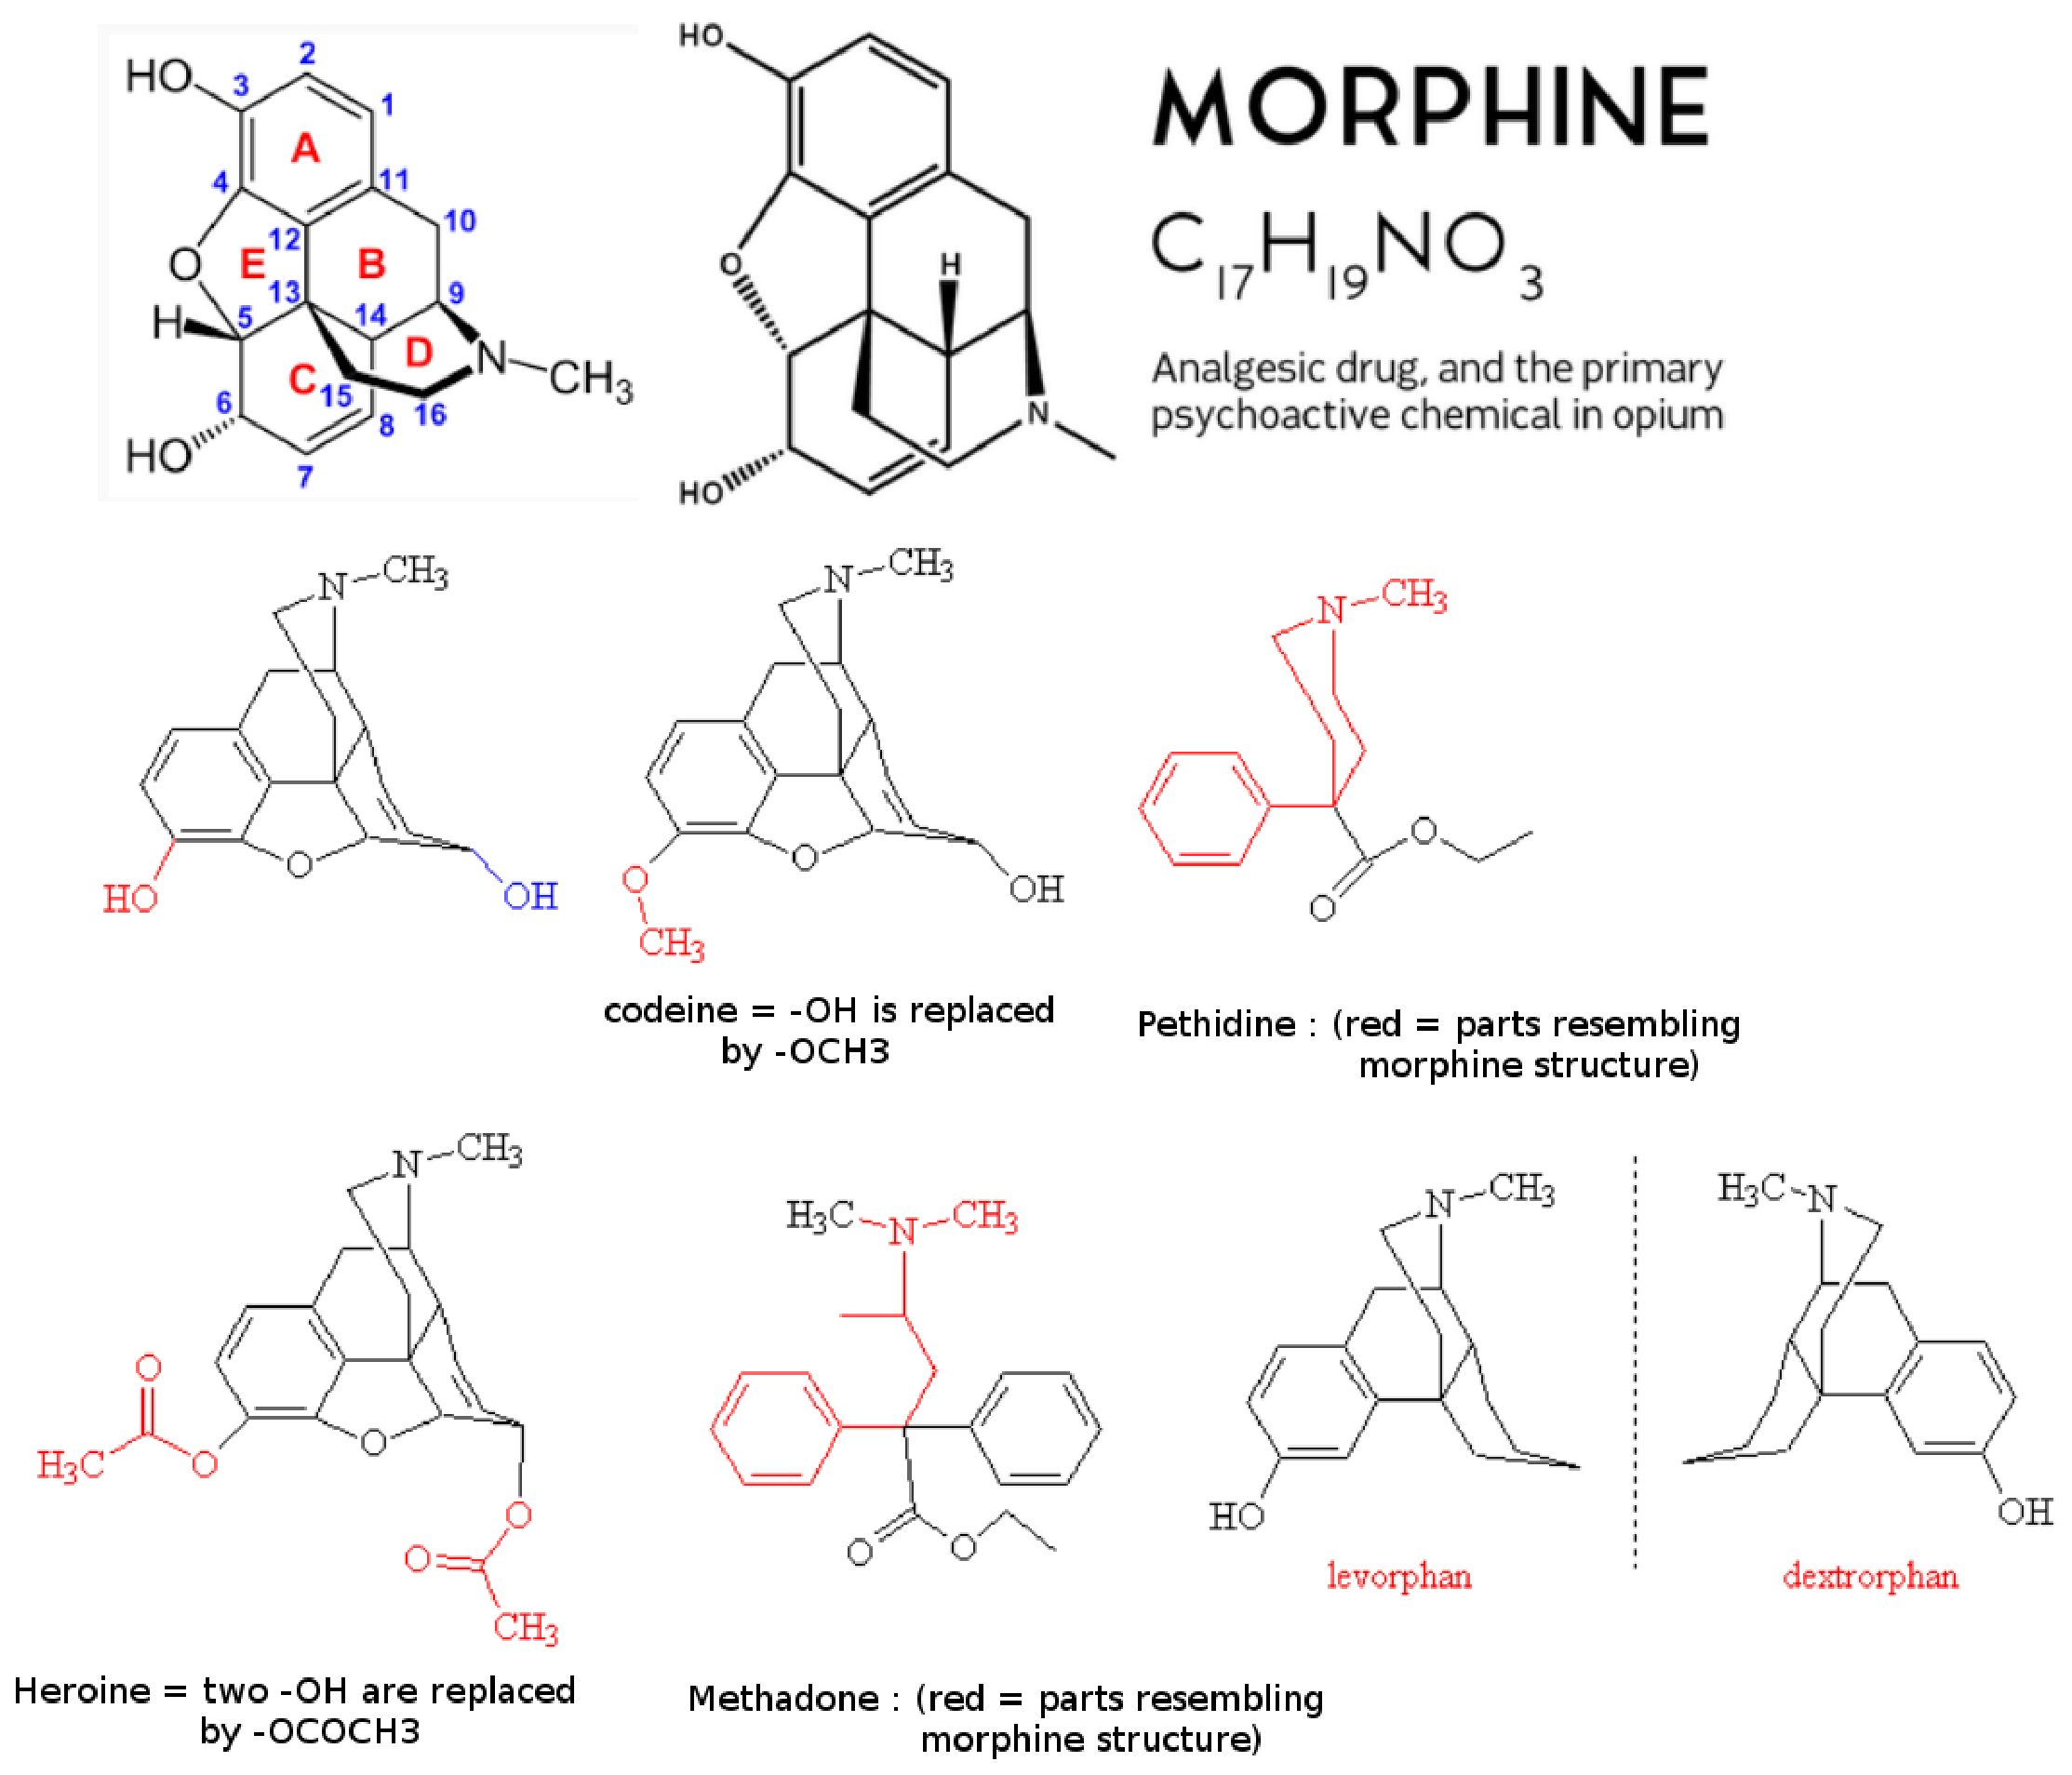
\includegraphics[height=8cm,
    angle=0]{./images/morphine.eps}}
  \caption{Morphine, Codeine, Pethidine, Heroine, Methadone}
\label{fig:morphine}
\end{figure}

The similar chemical structures, and these structural similarities lead to the
similar effects that these opioids have.


\subsection{codeine}
\label{sec:codeine}

Most commercial opium is converted into codeine by methylation,
Fig.\ref{fig:morphine}.
 

\subsection{side effect}

Morphine acts as an anesthetic without decreasing consciousness, and it is one
of the most powerful analgesics known. However it also suppresses the
respiratory system, and high doses can cause death by respiratory failure.

Morphine-like drugs work mostly on the brain and higher doses depress all
functions with depression of respiration being the major cause of death. 






